\documentclass{standalone}
\usepackage{tikz}
\usetikzlibrary{patterns, positioning}


\begin{document}
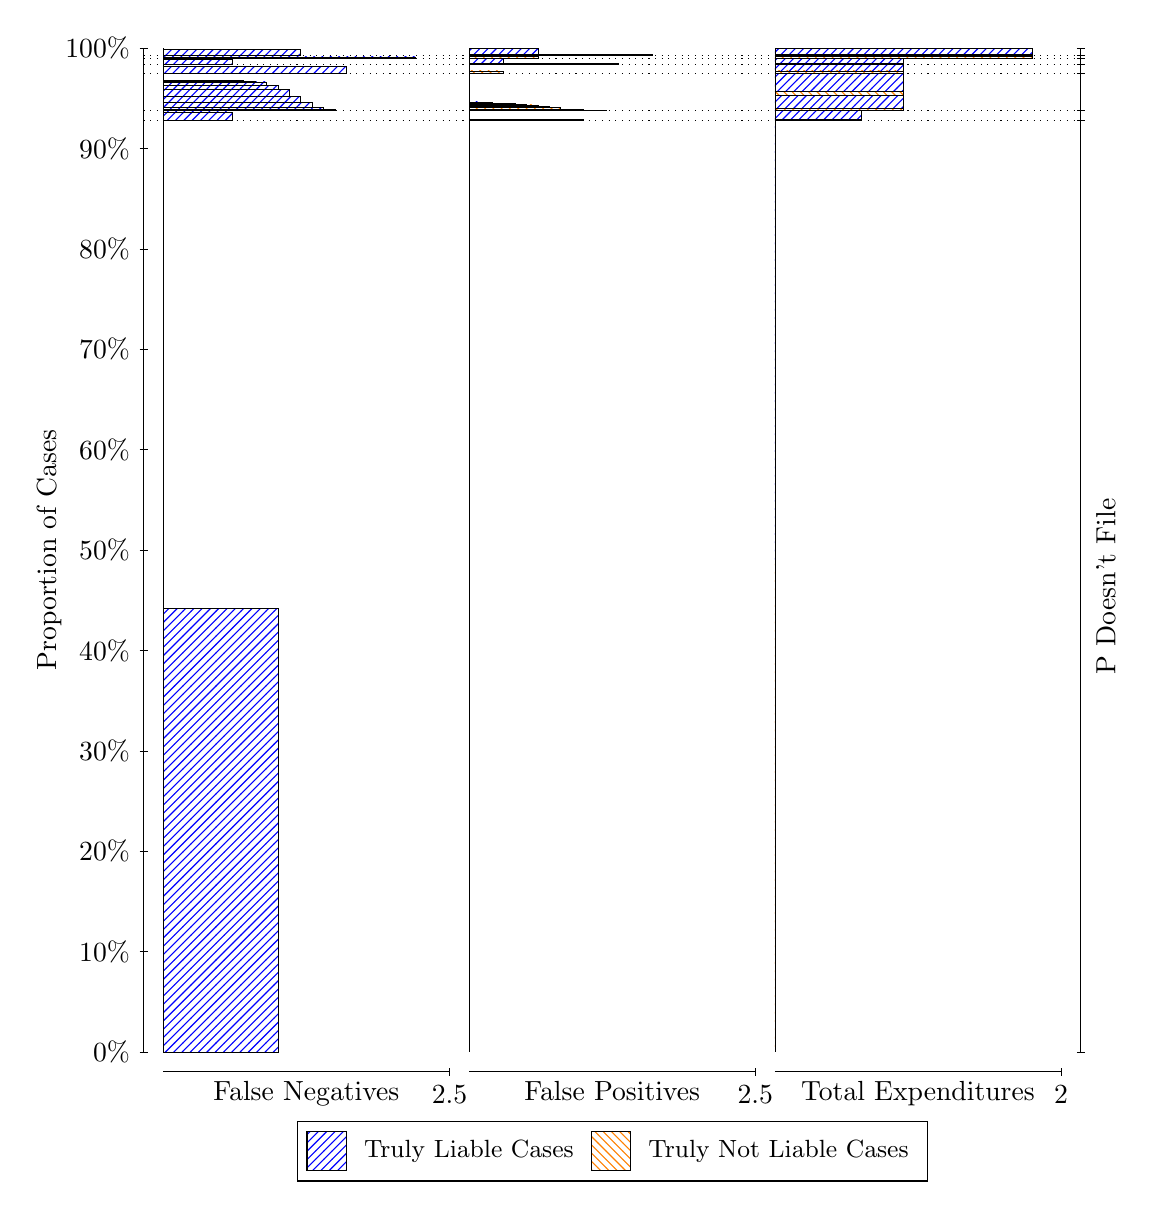
\begin{tikzpicture}
\draw[black, very thin] (1.5,1.75) -- (1.5,14.5);
\node[rotate=90, text=black, anchor=center] at (0.3, 8.125) {Proportion of Cases};
\draw[black, very thin] (1.45,1.75) -- (1.55,1.75);
\node[text=black, anchor=east] at (1.45, 1.75) {0\%};
\draw[black, very thin] (1.45,3.025) -- (1.55,3.025);
\node[text=black, anchor=east] at (1.45, 3.025) {10\%};
\draw[black, very thin] (1.45,4.3) -- (1.55,4.3);
\node[text=black, anchor=east] at (1.45, 4.3) {20\%};
\draw[black, very thin] (1.45,5.575) -- (1.55,5.575);
\node[text=black, anchor=east] at (1.45, 5.575) {30\%};
\draw[black, very thin] (1.45,6.85) -- (1.55,6.85);
\node[text=black, anchor=east] at (1.45, 6.85) {40\%};
\draw[black, very thin] (1.45,8.125) -- (1.55,8.125);
\node[text=black, anchor=east] at (1.45, 8.125) {50\%};
\draw[black, very thin] (1.45,9.4) -- (1.55,9.4);
\node[text=black, anchor=east] at (1.45, 9.4) {60\%};
\draw[black, very thin] (1.45,10.675) -- (1.55,10.675);
\node[text=black, anchor=east] at (1.45, 10.675) {70\%};
\draw[black, very thin] (1.45,11.95) -- (1.55,11.95);
\node[text=black, anchor=east] at (1.45, 11.95) {80\%};
\draw[black, very thin] (1.45,13.225) -- (1.55,13.225);
\node[text=black, anchor=east] at (1.45, 13.225) {90\%};
\draw[black, very thin] (1.45,14.5) -- (1.55,14.5);
\node[text=black, anchor=east] at (1.45, 14.5) {100\%};

\draw[black, very thin] (13.4,1.75) -- (13.4,14.5);
\draw[black, very thin] (13.35,1.75) -- (13.45,1.75);
\node[anchor=west] at (13.35, 1.75) {};
\draw[black, very thin] (13.35,13.578) -- (13.45,13.578);
\node[anchor=west] at (13.35, 13.578) {};
\draw[black, very thin] (13.35,13.706) -- (13.45,13.706);
\node[anchor=west] at (13.35, 13.706) {};
\draw[black, very thin] (13.35,14.179) -- (13.45,14.179);
\node[anchor=west] at (13.35, 14.179) {};
\draw[black, very thin] (13.35,14.296) -- (13.45,14.296);
\node[anchor=west] at (13.35, 14.296) {};
\draw[black, very thin] (13.35,14.372) -- (13.45,14.372);
\node[anchor=west] at (13.35, 14.372) {};
\draw[black, very thin] (13.35,14.404) -- (13.45,14.404);
\node[anchor=west] at (13.35, 14.404) {};
\draw[black, very thin] (13.35,14.5) -- (13.45,14.5);
\node[anchor=west] at (13.35, 14.5) {};

\draw[black, very thin, pattern color=blue, pattern=north east lines] (1.75,1.75) rectangle (3.2033,7.3792);
\draw[black, very thin, pattern color=orange, pattern=north west lines] (1.75,7.3792) rectangle (1.75,13.578);
\draw[black, very thin, pattern color=blue, pattern=north east lines] (1.75,13.578) rectangle (2.622,13.688);
\draw[black, very thin, pattern color=orange, pattern=north west lines] (1.75,13.688) rectangle (1.75,13.706);
\draw[black, very thin, pattern color=blue, pattern=north east lines] (1.75,13.706) rectangle (3.93,13.719);
\draw[black, very thin, pattern color=blue, pattern=north east lines] (1.75,13.719) rectangle (3.7847,13.742);
\draw[black, very thin, pattern color=blue, pattern=north east lines] (1.75,13.742) rectangle (3.6393,13.805);
\draw[black, very thin, pattern color=blue, pattern=north east lines] (1.75,13.805) rectangle (3.494,13.884);
\draw[black, very thin, pattern color=blue, pattern=north east lines] (1.75,13.884) rectangle (3.3487,13.973);
\draw[black, very thin, pattern color=blue, pattern=north east lines] (1.75,13.973) rectangle (3.2033,14.022);
\draw[black, very thin, pattern color=blue, pattern=north east lines] (1.75,14.022) rectangle (3.058,14.069);
\draw[black, very thin, pattern color=blue, pattern=north east lines] (1.75,14.069) rectangle (2.9127,14.08);
\draw[black, very thin, pattern color=blue, pattern=north east lines] (1.75,14.08) rectangle (2.7673,14.092);
\draw[black, very thin, pattern color=orange, pattern=north west lines] (1.75,14.092) rectangle (1.75,14.179);
\draw[black, very thin, pattern color=blue, pattern=north east lines] (1.75,14.179) rectangle (4.0753,14.266);
\draw[black, very thin, pattern color=orange, pattern=north west lines] (1.75,14.266) rectangle (1.75,14.296);
\draw[black, very thin, pattern color=blue, pattern=north east lines] (1.75,14.296) rectangle (2.622,14.362);
\draw[black, very thin, pattern color=orange, pattern=north west lines] (1.75,14.362) rectangle (1.75,14.372);
\draw[black, very thin, pattern color=blue, pattern=north east lines] (1.75,14.372) rectangle (4.9473,14.387);
\draw[black, very thin, pattern color=orange, pattern=north west lines] (1.75,14.387) rectangle (1.75,14.404);
\draw[black, very thin, pattern color=blue, pattern=north east lines] (1.75,14.404) rectangle (3.494,14.485);
\draw[black, very thin, pattern color=orange, pattern=north west lines] (1.75,14.485) rectangle (1.75,14.5);
\draw[black, very thin, pattern color=orange, pattern=north west lines] (5.6333,1.75) rectangle (5.6333,7.9488);
\draw[black, very thin, pattern color=blue, pattern=north east lines] (5.6333,7.9488) rectangle (5.6333,13.578);
\draw[black, very thin, pattern color=orange, pattern=north west lines] (5.6333,13.578) rectangle (7.0867,13.595);
\draw[black, very thin, pattern color=blue, pattern=north east lines] (5.6333,13.595) rectangle (5.6333,13.706);
\draw[black, very thin, pattern color=orange, pattern=north west lines] (5.6333,13.706) rectangle (7.3773,13.708);
\draw[black, very thin, pattern color=orange, pattern=north west lines] (5.6333,13.708) rectangle (7.232,13.709);
\draw[black, very thin, pattern color=orange, pattern=north west lines] (5.6333,13.709) rectangle (7.0867,13.717);
\draw[black, very thin, pattern color=orange, pattern=north west lines] (5.6333,13.717) rectangle (6.9413,13.725);
\draw[black, very thin, pattern color=orange, pattern=north west lines] (5.6333,13.725) rectangle (6.796,13.743);
\draw[black, very thin, pattern color=orange, pattern=north west lines] (5.6333,13.743) rectangle (6.6507,13.758);
\draw[black, very thin, pattern color=orange, pattern=north west lines] (5.6333,13.758) rectangle (6.5053,13.778);
\draw[black, very thin, pattern color=orange, pattern=north west lines] (5.6333,13.778) rectangle (6.36,13.788);
\draw[black, very thin, pattern color=orange, pattern=north west lines] (5.6333,13.788) rectangle (6.2147,13.793);
\draw[black, very thin, pattern color=blue, pattern=north east lines] (5.6333,13.793) rectangle (5.924,13.805);
\draw[black, very thin, pattern color=blue, pattern=north east lines] (5.6333,13.805) rectangle (5.7787,13.816);
\draw[black, very thin, pattern color=blue, pattern=north east lines] (5.6333,13.816) rectangle (5.6333,14.179);
\draw[black, very thin, pattern color=orange, pattern=north west lines] (5.6333,14.179) rectangle (6.0693,14.209);
\draw[black, very thin, pattern color=blue, pattern=north east lines] (5.6333,14.209) rectangle (5.6333,14.296);
\draw[black, very thin, pattern color=orange, pattern=north west lines] (5.6333,14.296) rectangle (7.5227,14.306);
\draw[black, very thin, pattern color=blue, pattern=north east lines] (5.6333,14.306) rectangle (6.0693,14.372);
\draw[black, very thin, pattern color=orange, pattern=north west lines] (5.6333,14.372) rectangle (6.5053,14.389);
\draw[black, very thin, pattern color=blue, pattern=north east lines] (5.6333,14.389) rectangle (5.6333,14.404);
\draw[black, very thin, pattern color=orange, pattern=north west lines] (5.6333,14.404) rectangle (7.9587,14.419);
\draw[black, very thin, pattern color=blue, pattern=north east lines] (5.6333,14.419) rectangle (6.5053,14.5);
\draw[black, very thin, pattern color=orange, pattern=north west lines] (9.5167,1.75) rectangle (9.5167,7.9488);
\draw[black, very thin, pattern color=blue, pattern=north east lines] (9.5167,7.9488) rectangle (9.5167,13.578);
\draw[black, very thin, pattern color=orange, pattern=north west lines] (9.5167,13.578) rectangle (10.607,13.595);
\draw[black, very thin, pattern color=blue, pattern=north east lines] (9.5167,13.595) rectangle (10.607,13.706);
\draw[black, very thin, pattern color=orange, pattern=north west lines] (9.5167,13.706) rectangle (11.152,13.738);
\draw[black, very thin, pattern color=blue, pattern=north east lines] (9.5167,13.738) rectangle (11.152,13.898);
\draw[black, very thin, pattern color=orange, pattern=north west lines] (9.5167,13.898) rectangle (11.152,13.953);
\draw[black, very thin, pattern color=blue, pattern=north east lines] (9.5167,13.953) rectangle (11.152,14.179);
\draw[black, very thin, pattern color=orange, pattern=north west lines] (9.5167,14.179) rectangle (11.152,14.209);
\draw[black, very thin, pattern color=blue, pattern=north east lines] (9.5167,14.209) rectangle (11.152,14.296);
\draw[black, very thin, pattern color=orange, pattern=north west lines] (9.5167,14.296) rectangle (11.152,14.306);
\draw[black, very thin, pattern color=blue, pattern=north east lines] (9.5167,14.306) rectangle (11.152,14.372);
\draw[black, very thin, pattern color=orange, pattern=north west lines] (9.5167,14.372) rectangle (12.787,14.389);
\draw[black, very thin, pattern color=blue, pattern=north east lines] (9.5167,14.389) rectangle (12.787,14.404);
\draw[black, very thin, pattern color=orange, pattern=north west lines] (9.5167,14.404) rectangle (12.787,14.419);
\draw[black, very thin, pattern color=blue, pattern=north east lines] (9.5167,14.419) rectangle (12.787,14.5);
\draw[black, dotted] (1.5,13.578) -- (13.4,13.578);
\draw[black, dotted] (1.5,13.706) -- (13.4,13.706);
\draw[black, dotted] (1.5,14.179) -- (13.4,14.179);
\draw[black, dotted] (1.5,14.296) -- (13.4,14.296);
\draw[black, dotted] (1.5,14.372) -- (13.4,14.372);
\draw[black, dotted] (1.5,14.404) -- (13.4,14.404);
\draw[black, very thin] (1.75,1.5) -- (5.3833,1.5);
\node[text=black, anchor=north] at (3.5667, 1.5) {False Negatives};
\draw[black, very thin] (5.3833,1.45) -- (5.3833,1.55);
\node[text=black, anchor=north] at (5.3833, 1.45) {2.5};

\draw[black, very thin] (5.6333,1.5) -- (9.2667,1.5);
\node[text=black, anchor=north] at (7.45, 1.5) {False Positives};
\draw[black, very thin] (9.2667,1.45) -- (9.2667,1.55);
\node[text=black, anchor=north] at (9.2667, 1.45) {2.5};

\draw[black, very thin] (9.5167,1.5) -- (13.15,1.5);
\node[text=black, anchor=north] at (11.333, 1.5) {Total Expenditures};
\draw[black, very thin] (13.15,1.45) -- (13.15,1.55);
\node[text=black, anchor=north] at (13.15, 1.45) {2};

\node[text=black, centered, rotate=90] at (13.72, 7.664) {P Doesn't File};







\draw (7.449999999999999,1.5) node[draw=none] (baseCoordinate) {};
\begin{scope}[align=center]
        \matrix[scale=0.5, draw=black, below=0.5cm of baseCoordinate, nodes={draw}, column sep=0.1cm]{
            \node[rectangle, draw, minimum width=0.5cm, minimum height=0.5cm, pattern color=blue, pattern=north east lines] {}; &
            \node[draw=none, font=\small, text=black] (B) {Truly Liable Cases}; &
            \node[rectangle, draw, minimum width=0.5cm, minimum height=0.5cm, pattern color=orange, pattern=north west lines] {}; &
            \node[draw=none, font=\small, text=black] (B) {Truly Not Liable Cases}; \\
            };
\end{scope}

\end{tikzpicture}
\end{document}